\documentclass[12pt,a4paper,oneside]{article}
\usepackage{amsmath,amsthm}
\usepackage{graphicx}
\usepackage{ctex}

\title{计算方法编程作业一实验报告}
\author{张博厚 PB22071354}
\date{}

\begin{document}
\maketitle

\section{实验内容}
本实验要求编程求解一反射问题的二维简化模型: 将镜面假定为圆形, 给定观察点P与物点Q, 
输出反射点T和像点R.

\section{算法}
\subsection{计算反射点T}
对于反射点T,参考《Computational Mirror Cup and Saucer Art》中的方法,使用二分法数值求解:
假定观察点P在x轴负半轴,物点Q在第二象限, P与Q均在圆外, G为过点P在第二象限内所作切线的
切点, 如图1所示.
\begin{figure}[htbp]
    \centering
    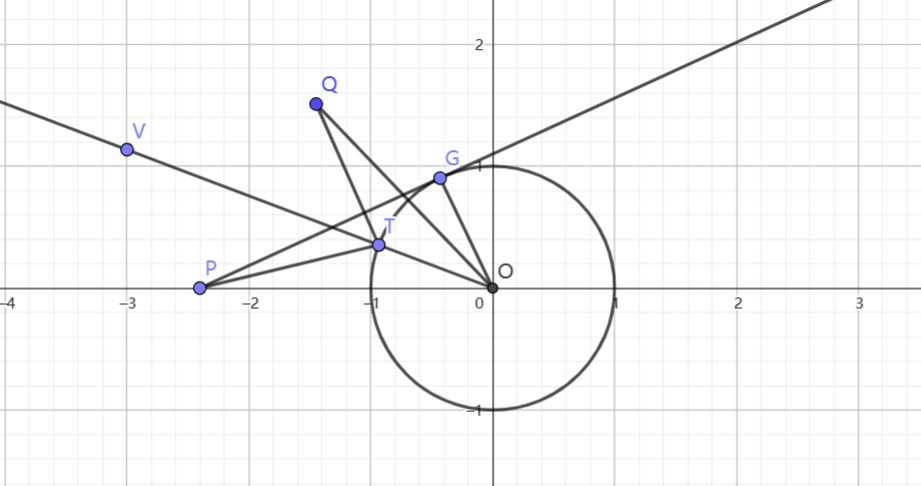
\includegraphics[width = 0.77\textwidth]{figs/f.png}
    \caption{反射模型及各点示意图}
\end{figure}\par
通过二分法确定$\angle POT$的大小,进而确定T的位置, 首先应分别计算$\angle POG, \angle POQ$
的大小:
$$\angle POG = \arccos{\dfrac{1}{\lvert x_P \rvert}}$$
$$  \angle POQ = \arccos{\dfrac{\lvert x_Q \rvert}{\sqrt{x_Q^2+y_Q^2}}}$$
用二分的方式,取初值$high=min\{\angle POG,\angle POQ\},\ low=0$,每次令
$\angle POT = \frac{1}{2}(low+high)$, 可知T的坐标为$(-\cos{\angle POT}, \sin{\angle POT})$.下面
分别计算$\angle PTV, \angle QTV$: 由T坐标可得直线OT方程:
\begin{equation}
    \sin{\angle POT}\ x+\cos{\angle POT}\ y=0
\end{equation}
故P,Q两点到直线OT的距离分别为
\begin{equation*}
    l_1 = \dfrac{\lvert \sin{\angle POT}\ x_P+\cos{\angle POT}\ y_P \rvert}{\sin{\angle POT}^2+\cos{\angle POT}^2 }
        =\lvert \sin{\angle POT}\ x_P+\cos{\angle POT}\ y_P \rvert
\end{equation*}
\begin{equation*}
    l_2 = \lvert \sin{\angle POT}\ x_Q+\cos{\angle POT}\ y_Q \rvert
\end{equation*}
于是
$$\angle PTV = \arcsin{\dfrac{l_1}{\lvert PT \rvert}}$$
$$\angle QTV = \arcsin{\dfrac{l_2}{\lvert QT \rvert}}$$
比较$\angle PTV$与$\angle QTV$的大小, 并据此调整二分的上限或下限, 直到两角误差在可接受的范围内
(实验中设置为double类型的精度15位), 此时的T即为所求反射点.

\subsection{计算像点R}
对于像点R, 在已知Q与T的前提下用解析法求解.
\end{document}